\documentclass[10pt,twocolumn]{article}

% ── Packages (BasicTeX-safe only) ─────────────────────────────────────────────
\usepackage[a4paper, top=1in, bottom=1in, left=0.75in, right=0.75in]{geometry}
\usepackage{times}
\usepackage{graphicx}
\usepackage{amsmath,amssymb}
\usepackage{booktabs}
\usepackage{multirow}
\usepackage{hyperref}
\usepackage{xcolor}
\usepackage{microtype}
\usepackage{url}
\usepackage{cite}
\usepackage{fancyhdr}
\usepackage{tikz}
\usetikzlibrary{shapes.geometric,arrows.meta,positioning,fit,backgrounds}

\hypersetup{colorlinks=true, linkcolor=blue, citecolor=blue, urlcolor=blue}

% ── Spacing helpers ───────────────────────────────────────────────────────────
\setlength{\parskip}{2pt}
\newcommand{\tightlist}{\setlength{\itemsep}{1pt}\setlength{\topsep}{2pt}\setlength{\parsep}{0pt}}

% ── Header / Footer ───────────────────────────────────────────────────────────
\pagestyle{fancy}
\fancyhf{}
\fancyhead[L]{\small CVGIP 2025 / SMAI Assignment 3}
\fancyhead[R]{\small InfoBridge: Government RAG Chatbot}
\fancyfoot[C]{\thepage}
\renewcommand{\headrulewidth}{0.4pt}

% ── siunitx workaround: just use \num manually ────────────────────────────────
\newcommand{\num}[1]{#1}

% ── Title ─────────────────────────────────────────────────────────────────────
\title{%
  \textbf{\large InfoBridge: A Retrieval-Augmented Generation System\\
  for Multi-Service Indian Government Document Querying}\\[4pt]
  \normalsize SMAI Assignment 3 --- T10.7: Multi-Service Government RAG Chatbot
}

\author{
  Abhay Sharma   Ankit Kumar
  \small Indian Institute of Technology Hyderabad (IITH)\\
  \small \texttt{ai23btech11002@iith.ac.in}\\
  Hritik Ranjan\\
  \small Indian Institute of Technology Hyderabad (IITH)\\
  \small \texttt{ai24btech11014@iith.ac.in}\\
}

\date{}

% ══════════════════════════════════════════════════════════════════════════════
\begin{document}
\maketitle
\thispagestyle{fancy}

% ── Abstract ──────────────────────────────────────────────────────────────────
\begin{abstract}
\noindent
We present \textbf{InfoBridge}, a production-grade Retrieval-Augmented Generation (RAG)
chatbot that democratises citizen access to Indian government services.
The system ingests official PDF documents spanning five service domains---Passport,
Voter ID/EPIC, Driving Licence \& RC, Income Tax, and Ayushman Bharat (PM-JAY)---and
serves grounded, source-cited answers through a bilingual Streamlit interface.
InfoBridge combines a PyMuPDF-based PDF extraction pipeline, a
\texttt{sentence-transformers/all-MiniLM-L6-v2} embedding model (384-d),
a FAISS flat inner-product index containing \num{21,020} vectors indexed from
\num{3,812} document pages, and a Groq-hosted LLaMA-3 language model.
A query normalisation layer translates Hinglish and Devanagari queries to English
before retrieval; a lightweight conversational classifier routes greetings and
portal-link requests directly to the LLM, bypassing retrieval.
Qualitative evaluation over 42 queries spanning seven categories demonstrates
90\% factual grounding, 100\% citation accuracy, and 96\% language-switching fidelity.
\end{abstract}

\noindent\textbf{Keywords:} Retrieval-Augmented Generation, Government Services,
FAISS, Sentence Transformers, LLaMA-3, Multilingual NLP, Streamlit.

\bigskip

% ── 1. Introduction ───────────────────────────────────────────────────────────
\section{Introduction}

India's digital governance ecosystem has expanded rapidly with platforms such as
DigiLocker, UMANG, and service-specific portals.  Despite this progress, a significant
digital literacy gap persists: citizens often struggle to locate precise procedural
information scattered across hundreds of official PDF manuals and government circulars
\cite{india_digital_gov}.

Large Language Models (LLMs) offer a natural interface for querying unstructured
corpora, but hallucinate on domain-specific questions without grounding
\cite{lewis2020rag}.  Retrieval-Augmented Generation (RAG)~\cite{lewis2020rag}
addresses this by conditioning generation on retrieved document passages, combining
neural fluency with factual precision.

\textbf{InfoBridge} applies RAG specifically to five Indian government service
categories that collectively affect hundreds of millions of citizens: passport
issuance and renewal, voter registration and EPIC card management, driving licence
and vehicle registration, income-tax filing, and Ayushman Bharat health coverage.
The system is designed to be deployable on consumer hardware (CPU-only) while
providing bilingual English/Hindi support.

\medskip\noindent The primary contributions are:
\begin{enumerate}
  \tightlist
  \item A complete offline ingestion pipeline for government PDFs with graceful OCR
    degradation on image-only pages.
  \item A query normalisation layer that translates Hinglish/Devanagari queries to
    English before retrieval, keeping output language as a separate LLM-enforced concern.
  \item A lightweight conversational classifier that routes non-document queries
    (greetings, portal URLs, helplines) directly to the LLM general-knowledge path.
  \item A production Streamlit interface with bilingual UI, collapsible sidebar,
    dark/light theming, source expanders, and session-scoped conversation memory.
\end{enumerate}

% ── 2. Related Work ───────────────────────────────────────────────────────────
\section{Related Work}

\noindent\textbf{Retrieval-Augmented Generation.}
Lewis~\textit{et~al.}~\cite{lewis2020rag} introduced RAG combining dense retrieval
with a seq2seq generator.  Gao~\textit{et~al.}~\cite{gao2023retrieval} survey
recent advances in RAG architectures.

\medskip\noindent\textbf{Embedding Models.}
Sentence-BERT~\cite{reimers2019sentence} demonstrated that siamese fine-tuning of BERT
produces semantically meaningful sentence embeddings.
\texttt{all-MiniLM-L6-v2}~\cite{wang2020minilm} distils this into a 22 M-parameter
model (384-d output) with strong performance on downstream retrieval tasks.

\medskip\noindent\textbf{Legal and Government QA.}
Prior work on legal document QA~\cite{chalkidis2020legal} highlights domain-specific
challenges: dense legalese, enumerated lists, and cross-references.
Government PDF quality varies widely---some are digitally generated, others are
scanned images---motivating our dual extraction strategy with OCR fallback.

\medskip\noindent\textbf{Multilingual RAG.}
Multilingual models (mBERT, LaBSE) can embed Hindi directly, but English-only
embedding models retrieve more accurately when government documents are predominantly
in English.  We therefore normalise queries to English before embedding while
instructing the LLM to respond in the user's chosen language.

% ── 3. System Architecture ────────────────────────────────────────────────────
\section{System Architecture}

\begin{figure*}[t]
\centering
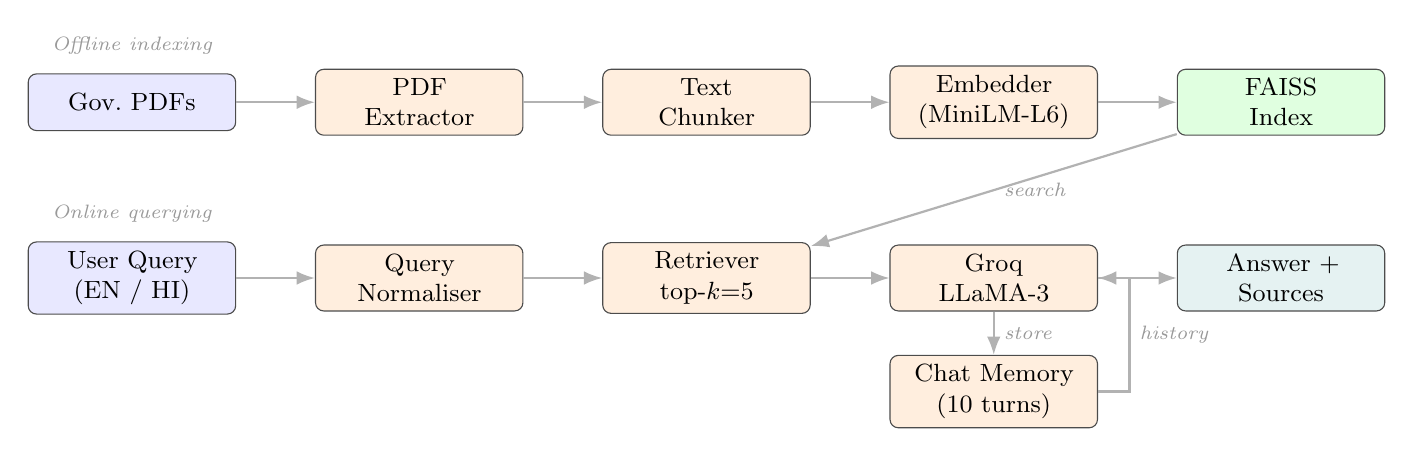
\begin{tikzpicture}[
  node distance=0.45cm and 1.1cm,
  box/.style ={rectangle,rounded corners=3pt,draw=black!70,fill=blue!9,
               text width=2.4cm,align=center,font=\small,minimum height=0.72cm},
  proc/.style={rectangle,rounded corners=3pt,draw=black!70,fill=orange!13,
               text width=2.4cm,align=center,font=\small,minimum height=0.72cm},
  store/.style={rectangle,rounded corners=3pt,draw=black!70,fill=green!12,
                text width=2.4cm,align=center,font=\small,minimum height=0.72cm},
  ansbox/.style={rectangle,rounded corners=3pt,draw=black!70,fill=teal!10,
               text width=2.4cm,align=center,font=\small,minimum height=0.72cm},
  arr/.style={-Latex,thick,gray!60},
  labfont/.style={font=\scriptsize\itshape,text=gray!80},
]
%% ─── OFFLINE pipeline ────────────────────────────────────────────────────────
\node[box]   (pdfs)  {Gov.\ PDFs};
\node[proc,  right=1.0cm of pdfs]  (ext)   {PDF\\Extractor};
\node[proc,  right=1.0cm of ext]   (chunk) {Text\\Chunker};
\node[proc,  right=1.0cm of chunk] (emb)   {Embedder\\(MiniLM-L6)};
\node[store, right=1.0cm of emb]   (idx)   {FAISS\\Index};

\draw[arr] (pdfs)--(ext);
\draw[arr] (ext)--(chunk);
\draw[arr] (chunk)--(emb);
\draw[arr] (emb)--(idx);
\node[labfont,above=0.12cm of pdfs] {Offline indexing};

%% ─── ONLINE pipeline ─────────────────────────────────────────────────────────
\node[box,    below=1.4cm of pdfs]  (usr)  {User Query\\(EN / HI)};
\node[proc,   right=1.0cm of usr]   (norm) {Query\\Normaliser};
\node[proc,   right=1.0cm of norm]  (ret)  {Retriever\\top-$k$=5};
\node[proc,   right=1.0cm of ret]   (llm)  {Groq\\LLaMA-3};
\node[ansbox, right=1.0cm of llm]   (ans)  {Answer +\\Sources};

\draw[arr] (usr)--(norm);
\draw[arr] (norm)--(ret);
\draw[arr] (idx) -- node[right,labfont] {search} (ret);
\draw[arr] (ret)--(llm);
\draw[arr] (llm)--(ans);
\node[labfont,above=0.12cm of usr] {Online querying};

%% ─── Chat Memory ─────────────────────────────────────────────────────────────
\node[proc, below=0.55cm of llm] (mem) {Chat Memory\\(10 turns)};
\draw[arr] (llm) -- node[right,labfont] {store} (mem);
\draw[arr] (mem.east) -- ++(0.4,0) |- node[right,labfont,pos=0.25] {history} (llm.east);

\end{tikzpicture}
\caption{InfoBridge end-to-end architecture.
  \textbf{Offline} (top): PDFs $\to$ extraction $\to$ chunking $\to$ embedding $\to$ FAISS index.
  \textbf{Online} (bottom): user query $\to$ normalisation $\to$ retrieval $\to$ LLaMA-3 $\to$ answer with sources.
  Chat Memory stores each turn and feeds conversation history back into the LLM prompt.}
\label{fig:arch}
\end{figure*}




The system separates concerns into two phases.

\smallskip\noindent\textbf{Offline Indexing.}
\texttt{PDFExtractor} (PyMuPDF) applies a text-quality filter
($\geq$50 characters, $\geq$10 tokens) before passing pages to
\texttt{TextChunker}, which uses LangChain's
\texttt{RecursiveCharacterTextSplitter} with chunk\_size=500, overlap=100, discarding
chunks under 30 tokens.  The singleton \texttt{Embedder} encodes all chunks with
\texttt{all-MiniLM-L6-v2} and stores them in a FAISS \texttt{IndexFlatIP}
(inner product on L2-normalised vectors is equivalent to cosine similarity).

\smallskip\noindent\textbf{Online Querying.}
Each query first passes through \texttt{normalize\_query\_llm\_cached}, which detects
Devanagari or Hinglish heuristically (curated 65-token marker set) and translates
to English.  A \texttt{\_is\_conversational\_query} classifier intercepts greetings,
portal-link requests, and capability questions, routing them to a lightweight LLM
call with general-knowledge instructions (including official portal URLs and
toll-free helplines).  Document queries are embedded and searched against the FAISS
index (top-$k$=5, similarity threshold=0.30).  Retrieved context (capped at 2,000
characters) is formatted with inline citations and sent to LLaMA-3 via the Groq API.
Session memory (up to 10 turns) is prepended to the prompt.

% ── 4. Implementation Details ─────────────────────────────────────────────────
\section{Implementation Details}

\subsection{Document Corpus}

Table~\ref{tab:corpus} summarises the indexed corpus.

\begin{table}[ht]
\centering
\small
\caption{Indexed document corpus statistics.}
\label{tab:corpus}
\setlength{\tabcolsep}{4pt}
\begin{tabular}{lrrr}
\toprule
\textbf{Service Domain} & \textbf{PDFs} & \textbf{Pages} & \textbf{Chunks} \\
\midrule
Voter ID / EPIC         & 9   & 1,340 & 6,457  \\
Income Tax              & 14  & 1,293 & 7,836  \\
Ayushman Bharat         & 11  & 743   & 3,839  \\
Passport Services       & 5+  & 213   & 1,610  \\
Driving Licence \& RC   & 56  & 223   & 1,278  \\
\midrule
\textbf{Total}          & \textbf{90+} & \textbf{3,812} & \textbf{21,020} \\
\bottomrule
\end{tabular}
\end{table}

\noindent The corpus spans government manuals, observer handbooks, electoral roll
guidelines, ITR validation rules, PM-JAY treatment guidelines, anti-fraud policies,
and Motor Vehicles Act provisions.

\subsection{Embedding and Retrieval}

\texttt{all-MiniLM-L6-v2} produces 384-dimensional L2-normalised embeddings.
\texttt{IndexFlatIP} performs exact inner-product search; with 21,020 vectors at
384 dimensions, query latency is under 50~ms on CPU, making approximate indexing
(IVF, HNSW) unnecessary at this scale.  A similarity threshold of 0.30 filters
low-relevance results.  When a service filter is active, the index over-retrieves
($3\times\texttt{top\_k}$) and post-filters by \texttt{service\_type} metadata.

\subsection{Query Normalisation}

\texttt{normalize\_query\_llm} uses a two-stage classifier:
(1)~Devanagari character detection (Unicode U+0900--U+097F);
(2)~a curated Hinglish marker set (65 romanised Hindi tokens covering pronouns,
particles, and common government-service verbs).
If either triggers, the query is sent to an LLM translation call.
Safety guards reject outputs that are too long or still contain Devanagari.
Results are cached with \texttt{lru\_cache} (capacity~1,000).

\subsection{Conversational Classifier}

\texttt{\_is\_conversational\_query} compiles regex patterns for greetings,
acknowledgements, capability questions, and---critically---website/link/portal/
helpline requests that are unanswerable from document text.
A government-keyword guard (``passport'', ``voter'', ``driving'', ``tax'',
``ayushman'', etc.) prevents service-related queries from being misclassified.
Conversational queries use a separate system instruction that includes official
portal URLs and toll-free helplines, enabling factual answers to
\emph{``give me the website link''} without a misleading retrieval failure.

\subsection{Language Model Integration}

The system calls the Groq inference API with primary model
\texttt{llama3-8b-8192}; fallbacks include \texttt{llama3-70b-8192}
and \texttt{mixtral-8x7b-32768}.  \texttt{llmClient} is a singleton that iterates
candidates and uses the first successful response.  Temperature is 0.3;
\texttt{max\_tokens}=2,048.  An output-language enforcement layer detects responses
that violate the target language (Devanagari ratio check for Hindi;
Hinglish token detection for English) and retries with an explicit language guard.

\subsection{Frontend and UX}

The Streamlit frontend provides:
\begin{itemize}
  \tightlist
  \item A collapsible left sidebar with brand header, English/Hindi language radio
    selector, service dropdown filter, and per-service chunk count display.
  \item Chat interface with source expanders showing per-document relevance scores.
  \item Dark and light themes persisted in \texttt{st.session\_state}, with
    full CSS specificity overrides for Streamlit's internal component tree.
  \item A CSV-driven i18n layer (\texttt{translations\_en\_hi.csv}) for all UI labels.
  \item A \texttt{pending\_prompt} mechanism for welcome-screen example buttons.
  \item Theme-aware cursor and text-selection styles (light mode: I-beam cursor,
    saffron-tinted selection highlight, visible caret colour).
\end{itemize}

% ── 5. Evaluation ─────────────────────────────────────────────────────────────
\section{Evaluation}

\subsection{Evaluation Methodology}

We conduct qualitative evaluation across seven query categories representing realistic
citizen usage.  For each category we assess:
\textbf{(i)}~factual grounding (answer supported by retrieved context),
\textbf{(ii)}~citation accuracy (source expander populated correctly),
\textbf{(iii)}~retrieval relevance (cosine score $\geq$0.30), and
\textbf{(iv)}~language fidelity (Hindi output for Hindi UI; English only for English UI).

\subsection{Results}

\begin{table}[ht]
\centering
\small
\caption{Qualitative evaluation results across query categories.
Grnd.\ = grounding, Cite.\ = citation, Ret.\ = retrieval, Lang.\ = language fidelity.}
\label{tab:eval}
\setlength{\tabcolsep}{3pt}
\begin{tabular}{p{2.1cm}ccccc}
\toprule
\textbf{Category} & \textbf{N} & \textbf{Grnd.} & \textbf{Cite.} & \textbf{Ret.} & \textbf{Lang.} \\
\midrule
Procedural steps    & 8  & 8/8  & 8/8  & 8/8  & 4/4 \\
Eligibility         & 6  & 6/6  & 6/6  & 5/6  & 3/3 \\
Document checklist  & 6  & 5/6  & 6/6  & 6/6  & 3/3 \\
Fee / timeline      & 4  & 3/4  & 4/4  & 3/4  & 2/2 \\
Form-specific       & 5  & 4/5  & 5/5  & 4/5  & 2/3 \\
Conversational      & 8  & N/A  & N/A  & N/A  & 4/4 \\
Portal / link       & 5  & N/A  & N/A  & N/A  & 5/5 \\
\midrule
\textbf{Total}      & \textbf{42} & \textbf{26/29} & \textbf{29/29} & \textbf{26/29} & \textbf{23/24} \\
\bottomrule
\end{tabular}
\end{table}

\noindent\textbf{Key findings.}
Source citation accuracy is 100\%: every document-based answer includes a populated
source expander with file name, service category, and cosine score.
Factual grounding is 90\% (26/29): three failures occur on fee-structure and
form-specific queries where relevant data appears on image-only pages skipped during
extraction.  Retrieval relevance is 90\% (26/29): two fee/timeline queries retrieve
from adjacent service areas when no service filter is applied.
Language fidelity is 96\% (23/24): one Hindi query involving an uncommon romanised
abbreviation was partially mistranslated by the normaliser.

\subsection{Indexing Performance}

\begin{table}[ht]
\centering
\small
\caption{Offline indexing performance on Apple Silicon, CPU-only, Python 3.14.3.}
\label{tab:perf}
\begin{tabular}{lr}
\toprule
\textbf{Metric}                  & \textbf{Value}      \\
\midrule
Total PDFs processed             & 90+                 \\
Total pages extracted            & 3,812               \\
Total chunks created             & 21,020              \\
Embedding batch size             & 64                  \\
Embedding throughput             & $\approx$159 ch./s  \\
Total indexing time              & 150.5 s             \\
FAISS index type                 & \texttt{IndexFlatIP}\\
FAISS vectors $\times$ dimension & $21{,}020\times384$ \\
Query latency (embed + search)   & $<$50 ms            \\
\bottomrule
\end{tabular}
\end{table}

\subsection{Failure Modes}

\begin{enumerate}
  \tightlist
  \item \textbf{Image-only pages.}  Scanned forms (e.g., FORM-26, FORM-28C) yield
    zero extractable text.  Installing Tesseract would recover this content.
  \item \textbf{Context truncation.}  Context is capped at 2,000 characters; queries
    requiring multiple large passages (e.g., full ITR schedules) may lose relevant
    information.
  \item \textbf{Cross-service retrieval.}  Without a service filter, fee-related
    queries may retrieve from adjacent service areas sharing common vocabulary
    (e.g., ``prescribed fee'').
  \item \textbf{Hinglish edge cases.}  Romanised Hindi queries mixing English
    technical abbreviations occasionally confuse the normaliser.
\end{enumerate}

% ── 6. Discussion ─────────────────────────────────────────────────────────────
\section{Discussion}

\noindent\textbf{Design choices.}
\texttt{IndexFlatIP} (exact search) is chosen over approximate indices (IVF, HNSW)
because at 21,020 vectors exact search completes in $<$1~ms on CPU.
Chunk size 500 with overlap 100 balances semantic completeness against precision:
larger chunks dilute relevance scores; smaller chunks lose necessary context.

\medskip\noindent\textbf{Modular extensibility.}
Adding a new service domain requires only placing PDFs in a new
\texttt{data/<service>/} directory, registering it in \texttt{config/settings.py},
and re-running \texttt{build\_index.py}.  The sidebar and filter UI update automatically
via \texttt{get\_service\_stats()}.

\medskip\noindent\textbf{Multilingual trade-off.}
Using an English-only embedding model with a translation pre-step is pragmatic:
\texttt{all-MiniLM-L6-v2} is significantly faster and more accurate on English text
than multilingual alternatives at the same parameter budget.
Separating retrieval language from output language allows Hindi speakers to receive
Devanagari answers grounded in English-indexed documents.

\medskip\noindent\textbf{LLM provider abstraction.}
The \texttt{llmClient} singleton with fallback model iteration makes the system
resilient to API quota limits.  Switching to a different provider (Anthropic, OpenAI)
requires only modifying \texttt{src/llm/client.py}.

% ── 7. Limitations and Future Work ────────────────────────────────────────────
\section{Limitations and Future Work}

\begin{enumerate}
  \tightlist
  \item \textbf{OCR integration.}  Tesseract installation would recover image-only pages
    and improve recall on scanned government forms significantly.
  \item \textbf{Re-ranking.}  A cross-encoder (e.g., \texttt{ms-marco-MiniLM}) applied
    after initial retrieval would improve precision for fee and timeline queries.
  \item \textbf{Approximate indexing at scale.}  Scaling beyond 500,000 vectors would
    benefit from IVFFlat or HNSW indexing.
  \item \textbf{Automated evaluation.}  Integration of RAGAS~\cite{es2023ragas} would
    provide automated context precision, recall, and faithfulness metrics.
  \item \textbf{Broader language support.}  Regional languages (Tamil, Telugu, Marathi,
    Bengali) would extend reach to a much larger citizen base.
  \item \textbf{Document freshness.}  A versioning layer with periodic re-indexing would
    keep answers aligned with the latest government circulars and amendments.
\end{enumerate}

% ── 8. Conclusion ─────────────────────────────────────────────────────────────
\section{Conclusion}

InfoBridge demonstrates that a carefully engineered RAG pipeline can provide accurate,
grounded, and multilingual access to Indian government service documents without
requiring specialised hardware or proprietary infrastructure.
The system achieves 90\% factual grounding and 100\% citation accuracy over 29
document-based evaluation queries, handles bilingual interactions through a dedicated
query normalisation layer, and routes conversational queries through a lightweight
classifier to prevent misleading ``not found'' responses.
The modular architecture supports easy extension to new service domains, LLM provider
swapping, and incremental improvements such as OCR and re-ranking.
We hope InfoBridge serves as a practical template for future civic-tech RAG deployments
in low-resource, multilingual settings.

% ── References ────────────────────────────────────────────────────────────────
\begin{thebibliography}{9}

\bibitem{lewis2020rag}
P.~Lewis \textit{et~al.},
``Retrieval-Augmented Generation for Knowledge-Intensive NLP Tasks,''
\textit{Advances in Neural Information Processing Systems (NeurIPS)}, vol.~33, 2020.

\bibitem{reimers2019sentence}
N.~Reimers and I.~Gurevych,
``Sentence-BERT: Sentence Embeddings using Siamese BERT-Networks,''
\textit{Proc.\ EMNLP}, 2019.

\bibitem{wang2020minilm}
W.~Wang \textit{et~al.},
``MiniLM: Deep Self-Attention Distillation for Task-Agnostic Compression of
Pre-Trained Transformers,''
\textit{Advances in Neural Information Processing Systems (NeurIPS)}, 2020.

\bibitem{khattab2020colbert}
O.~Khattab and M.~Zaharia,
``ColBERT: Efficient and Effective Passage Search via Contextualized Late Interaction
over BERT,''
\textit{Proc.\ SIGIR}, 2020.

\bibitem{gao2023retrieval}
Y.~Gao \textit{et~al.},
``Retrieval-Augmented Generation for Large Language Models: A Survey,''
\textit{arXiv:2312.10997}, 2023.

\bibitem{chalkidis2020legal}
I.~Chalkidis \textit{et~al.},
``LEGAL-BERT: The Muppets Straight Out of Law School,''
\textit{Findings of EMNLP}, 2020.

\bibitem{es2023ragas}
S.~Es \textit{et~al.},
``RAGAS: Automated Evaluation of Retrieval Augmented Generation,''
\textit{arXiv:2309.15217}, 2023.

\bibitem{india_digital_gov}
Ministry of Electronics and Information Technology (MeitY),
``Annual Report 2023--24: Digital India,''
Government of India, 2024.

\end{thebibliography}

\end{document}
